\chapter{Acknowledgements}

% NOTE: pagestyle 放在 english 环境外面,否则无作用

\pagestyle{english}

% \begin{english}
{\englinespread

\begin{center}
    This fanfiction is based on \emph{Fallout: Equestria} by Kkat.    
\end{center}

\section*{Author}

\begin{center}
    Mimezinga
\end{center}

\section*{Cover by}

\begin{center}
    LimreiArt\footnote{\url{https://www.deviantart.com/limreiart/art/Pink-Eyes-513444372}}
\end{center}

\section*{Illustrations by}

\begin{center}
    Boiler3\footnote{\url{https://www.deviantart.com/boiler3/}}
\end{center}

\section*{Speical Thanks for Writing}

\begin{table}[H]
    \centering
    \begin{tabular}{ccc}
        Nyerguds & Damhoof & Easteu \\
        Aerondight & Arcane Scroll & Palacioskw \\
        Anonsamurai & & \\
    \end{tabular}
\end{table}

\section*{Typeset by}

\begin{center}
    RandomQuantum
\end{center}

\section*{Special Thanks for Typesetting}

\begin{table}[H]
    \centering
    
    \begin{center}
    Chinese \TeX{} Society\footnotemark and C\TeX{} Fourm\footnotemark
    \end{center}
  
    \begin{tabular}{rl}
        Ruixi Zhang & \texttt{@RuixiZhang42} \\
        Xiangdong Zeng & \texttt{@stone-zeng} \\
        Mu Zi & \texttt{@muzimuzhi} \\
        Zeping Lee & \texttt{@zepinglee} \\
        ChenCheng Huang & \texttt{@Liam0205} \\
    \end{tabular}
\end{table}

\addtocounter{footnote}{-2} % -2
\stepcounter{footnote}\footnotetext{\url{https://github.com/CTeX-org}}
\stepcounter{footnote}\footnotetext{\url{https://github.com/CTeX-org/forum/}}



\section*{Links}

\begin{itemize}
    \item Published on Fimfiction: \url{https://www.fimfiction.net/story/931/fallout-equestria-pink-eyes}
    \item English Ducument: \url{http://book.fallout-equestria.com/forum/viewtopic.php?f=3\&t=342}
    \item This Project on GitHub: \url{https://github.com/Ranqumn/FoE_pink_eyes_publish}
\end{itemize}

}
% \end{english}

% --------------------

\chapter{致谢}

\pagestyle{chinese}

\section*{译者}

\begin{center}
    MadCatMKII
\end{center}

\section*{初版制作}

\begin{table}[H]
    \centering
    \begin{tabular}{rl}
        NightScream & 校对 \\
        ShadowDumb & 校对\ 排版 \\
        NightlySound & 润色 \\
    \end{tabular}
\end{table}

\section*{特别感谢}

\begin{center}
    立冬 \quad Onisk
\end{center}

\section*{重排版制作}

\begin{center}
    RandomQuantum
\end{center}

\section*{专业排版特别感谢}

\begin{table}[H]
    \centering

    \begin{center}
    中文 \TeX{} 学会\footnotemark 与 C\TeX{} 论坛\footnotemark
    \end{center}

    \begin{tabular}{rl}
        张瑞熹 & \texttt{@RuixiZhang42} \\
        曾祥东 & \texttt{@stone-zeng} \\
        慕\mbox{\hspace{\ccwd}}子 & \texttt{@muzimuzhi} \\
        李泽平 & \texttt{@zepinglee} \\
        黄晨成 & \texttt{@Liam0205} \\
    \end{tabular}
\end{table}

\addtocounter{footnote}{-2} % -2
\stepcounter{footnote}\footnotetext{\url{https://github.com/CTeX-org}}
\stepcounter{footnote}\footnotetext{\url{https://github.com/CTeX-org/forum/}}


\section*{相关链接}

\begin{itemize}
    \item 作者原文地址 \url{https://www.fimfiction.net/story/931/fallout-equestria-pink-eyes}
    \item 英文电子文档 \url{http://book.fallout-equestria.com/forum/viewtopic.php?f=3\&t=342}
    \item 译文首发地址 \url{http://blog.sina.com.cn/u/3149389173}
    \item 完整译文地址 \url{https://fimtale.com/t/2387\#/radiant-ponies-pink-eyes}
    \item 印刷初版首发地址 \url{https://www.equestriacn.com/}
    \item 重排版项目地址 \url{https://github.com/Ranqumn/FoE_pink_eyes_publish}
    \item 封面首发地址 \url{https://www.deviantart.com/limreiart/art/Pink-Eyes-513444372}
    \item 插图 Boiler3 \url{https://www.deviantart.com/boiler3/}
\end{itemize}

% TODO: 添加地址


\clearpage

% ---------

% 手动调整

\fancyhf{} % 清空

\fancyhead[LE,RO]{\thepage}

\fancyhead[LO]{\sffamily \uppercase{Acknowledgements}} % 奇数页  \leftmark = 章节名称
\fancyhead[RE]{\sffamily \uppercase{Fallout Equestria: Pink Eyes}} % 偶数页

% 

~\vfill

\section*{The Last Special Thanks}

\begin{center}

    \Large You

\end{center}

~\vfill

\clearpage


~\vfill

\begin{center}

\begin{englishpar}
    \sout{Press any key to skip credits}
    
    (This function has not been provided yet)
\end{englishpar}

\CJKsout{按任意键跳过制作人员列表}

(暂不支持该功能)

\begin{englishpar}
    Thank you for playing \emph{Fallout Equestria: Pink Eyes}
\end{englishpar}

感谢您玩赏
\end{center}

~\vfill

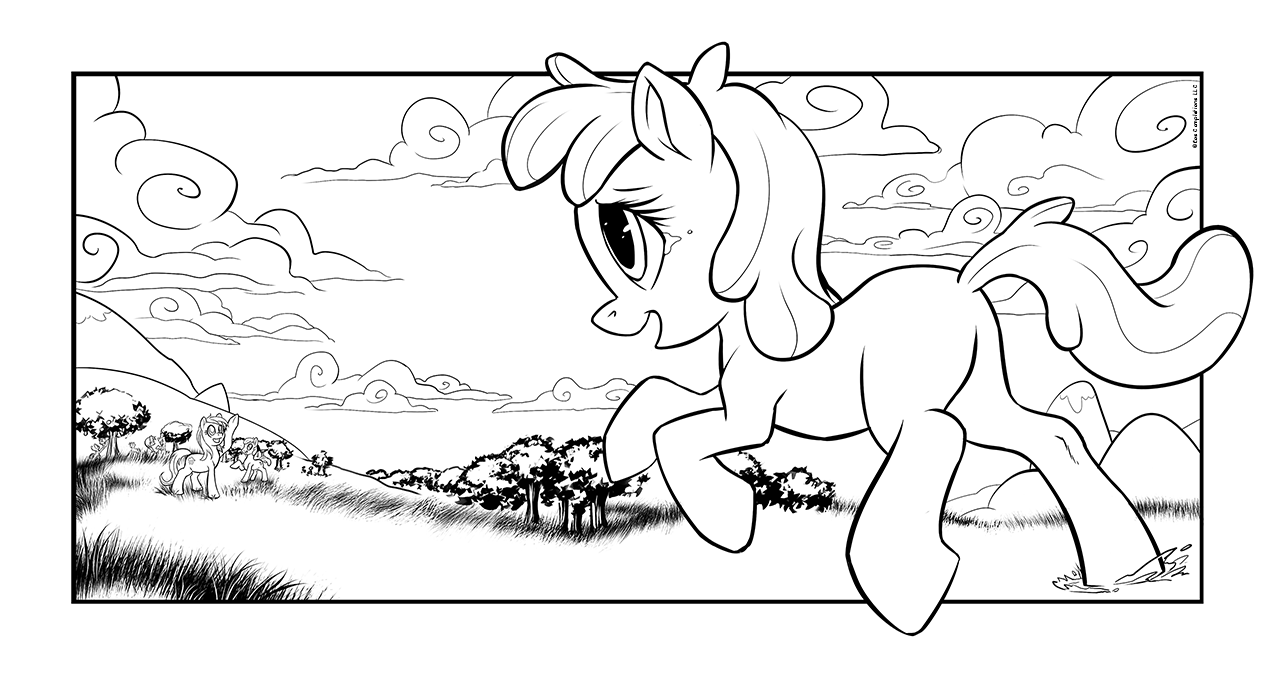
\includegraphics[width=0.9\linewidth]{image22.png}

\begin{motto}
    Do you believe in ghosts?

    你相信幽灵吗?
\end{motto}

